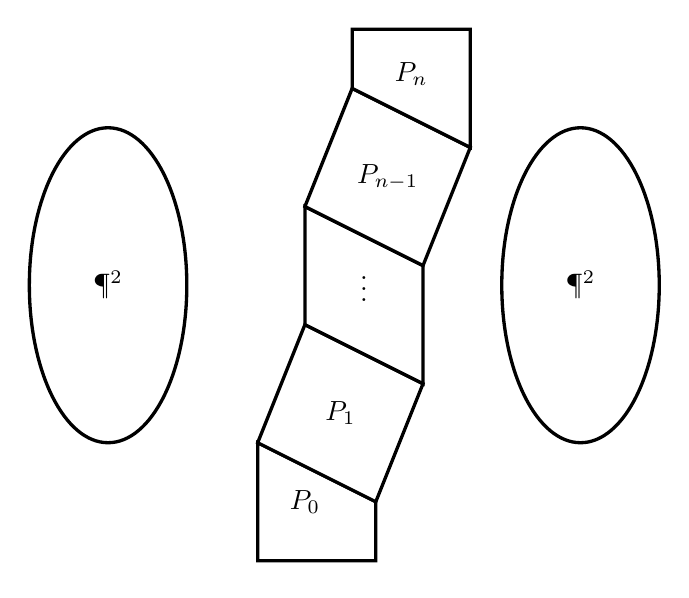
\begin{tikzpicture}[very thick]
  \begin{scope}[xshift=-3cm]
    \draw (0,0) ellipse (1 and 2);
    \draw (0,0) node {$\P^2$};
  \end{scope}
  \begin{scope}[yshift=-2cm, xshift=-0.5cm, yscale=0.75, xscale=1.5]
    \draw[fill=white] (-0.4,-2.0) -- (0.6,-2.0) -- (0.6, -1) -- (-0.4,0) -- cycle;
    \draw[fill=white] (0.6, -1) -- (-0.4,0) -- (0, 2) -- (1,1) -- cycle;
    \draw[fill=white] (0, 2) -- (1,1) -- (1,3) -- (0,4) -- cycle;
    \draw[fill=white] (1, 3) -- (0,4) -- (0.4, 6) -- (1.4,5) -- cycle;
    \draw[fill=white] (0.4, 6) -- (1.4,5) -- (1.4,7) -- (0.4,7) -- cycle;
    \draw
    (0,-1.0) node {$P_0$}
    (0.3,0.5) node {$P_1$}
    (0.5, 2.75) node {$\vdots$}
    (0.7, 4.5) node {$P_{n-1}$}
    (0.9, 6.25) node {$P_{n}$};
    \draw (0,-2) node (X) {};
  \end{scope}
  \begin{scope}[xshift=+3cm]
    \draw (0,0) ellipse (1 and 2);
    \draw (0,0) node {$\P^2$};
  \end{scope}
\end{tikzpicture}
%%% Local Variables:
%%% mode: latex
%%% TeX-master: "../main"
%%% End:
